\documentclass[openany]{book}

\usepackage{fancyhdr} % For style
\usepackage{geometry} % For margins
\usepackage{tocloft} % For TOC dots
\usepackage{multicol} % For multiple columns
\usepackage{graphicx} % For incorporating pictures

\geometry{margin=1in, headsep=30pt}
\pagestyle{fancy}

\renewcommand{\cftchapleader}{\cftdotfill{\cftdotsep}}

% "recipes.sty" package starts here:
\newcommand{\recipe}[1]{%
    \newpage
    \ichapter{#1}
    \chead{\Huge \bf{#1}}}%

\newcommand{\preptime}[1]{%
    \lhead{Prep time: #1}}

\newcommand{\cooktime}[1]{%
    \rhead{Cook time: #1}}

\newcommand{\ingredients}[1][\textbf{\Large\emph{Ingredients}}]{%
    \begin{center} \emph{#1} \end{center}}

\newcommand{\instructions}[1][
    \textbf{\Large\emph{Instructions}}]{%
    \begin{center}
    \emph{#1}
    \end{center}}%

\newcommand{\temp}[1]{%
    $#1^\circ$F}

% Cover Page
\title{Recipes}
\author{Brad Hall}
\date{}


\newcommand\ichapter[1]{%
  \refstepcounter{chapter}%
  \addcontentsline{toc}{chapter}{\protect\numberline{\thechapter}#1}%
  \sectionmark{#1}}

\begin{document}
\maketitle
\tableofcontents
\newpage

\recipe{Beef Stew}
\preptime{15 min}
\cooktime{2 hrs 40 mins}

\begin{multicols}{2}
\ingredients
\begin{itemize}
    \item 2.4lb chuck beef (cut into 3.5 cm/1.5'' cubes)
    \item 1 tsp each salt and pepper
    \item 3 tbsp olive oil (divided)
    \item 1 large onion (cut finely)
    \item 4 garlic cloves (minced)
    \item 3 carrots (cut into 2.5 cm/1'' pieces)
    \item 2 celery stalks (cut into 2.5 cm/1'' pieces)
    \item 1/3 cup flour
    \item 5 cups beef broth
    \item 2 tsp Worcestershire sauce
    \item 2 tbsp tomato paste
    \item 400 g/14 oz baby potatos (halved or quartered)
    \item More salt and pepper (to taste)
\end{itemize}

\vfill\null
\columnbreak

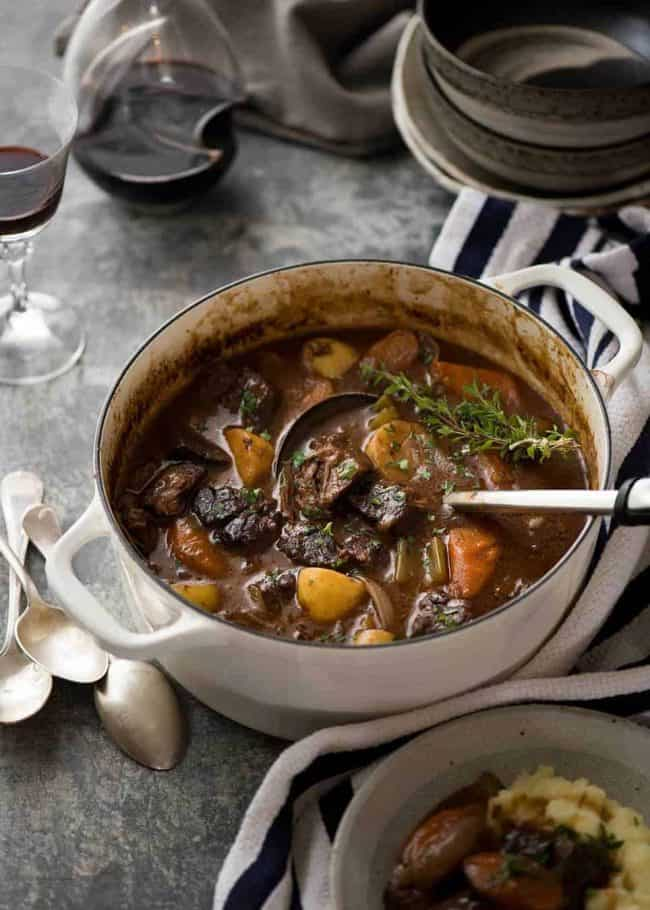
\includegraphics[height=8.75cm, width=7.5cm]{Pictures/Beef_Stew.jpg}
\end{multicols}

\instructions
\begin{enumerate}
    \item Sprinkle beef with salt and pepper.
    \item Heat 1 1/2 tbsp oil in a large, heavy based casserole pot over high heat until just starting to smoke.
    \item Add 1/3 of the beef and brown aggressively all over - about 4 minutes. Remove to bowl, repeat with remaining beef, adding more oil if required.
    \item Turn down heat to medium high. Add 1 tbsp oil if required. Add onion and garlic, cook for 2 minutes until onion is softened slightly and golden on the edge.
    \item Add carrot and celery, stir for 1 minute to coat in flavours.
    \item Sprinkle flour evenly across surface, then stir to coat.
    \item Add broth, tomato paste and Worcestershire sauce. Stir to dissolve tomato paste and flour into liquid.
    \item Add cooked beef (including any juices) and potato. Stir. Water level should almost fully cover everything, if not, add a touch of water.
    \item Bring to simmer, then adjust heat to low/medium low so it's simmering gently.
    \item Cover and cook for 1 hour 45 minutes or until beef is pretty tender (check with 2 forks at 1.5 hrs).
    \item Remove lid and simmer for further 30 minutes or until sauce reduces slightly. It should be like a thin gravy and beef should now be very tender.
    \item Season to taste with salt and pepper. 
    \item Serve over creamy mashed potato.
\end{enumerate}

\recipe{Meatloaf}
\preptime{10 min}
\cooktime{1 hr}

\begin{multicols}{2}
\ingredients
\begin{itemize}
    \item 1 1/2 lb ground beef
    \item 1 egg
    \item 1 onion (chopped)
    \item 1 cup milk
    \item 1 cup dried bread crumbs
    \item salt and pepper 
    \item 2 tbsp brown sugar
    \item 2 tbsp prepared mustard
    \item 1/3 cup ketchup
\end{itemize}

\vfill\null
\columnbreak

\hspace{-2cm}
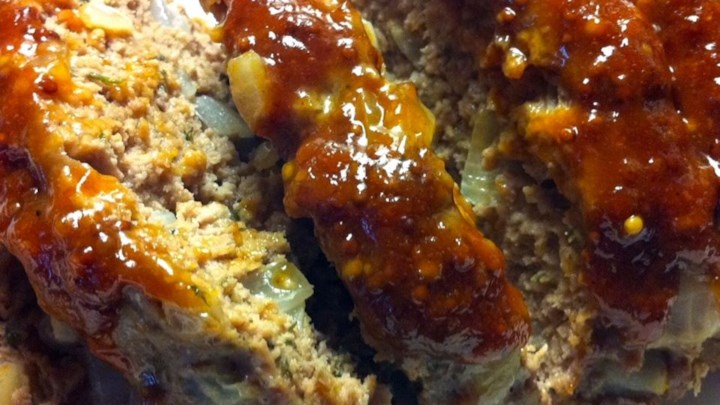
\includegraphics[height=8.75cm, width=9.75cm]{Pictures/Meatloaf.jpg}
\end{multicols}

\instructions
\begin{enumerate}
    \item Preheat oven to \temp{350}.
    \item In a large bowl, combine the beef, egg, onion, milk and bread crumbs. Season with salt and pepper to taste and place in a lightly greased 5x9 inch loaf pan (or form into a loaf and place in a lightly greased 9x13 inch baking dish).
    \item In a separate small bowl, combine the brown sugar, mustard and ketchup. Mix well and pour over the meatloaf.
    \item Bake at \temp{350} for 1 hour.
\end{enumerate}
\end{document}
